% #######################################
% ########### FILL THESE IN #############
% #######################################
\def\mytitle{Coursework Assessment 1}
\def\mykeywords{Oliver, Thornewill, Von, Essen, HTML, CSS, JavaScript, Web, Technologies, Napier}
\def\myauthor{Oliver Thornewill von Essen}
\def\contact{40210534@napier.ac.uk}
\def\mymodule{Web Technologies (SET08101)}
% #######################################
% #### YOU DON'T NEED TO TOUCH BELOW ####
% #######################################
\documentclass[10pt, a4paper]{article}
\usepackage[a4paper,top=1.75cm,bottom=1.5cm,left=4cm, right=4cm]{geometry}
\onecolumn
\usepackage{graphicx}
\graphicspath{{./images/}}
%colour our links, remove weird boxes
\usepackage[colorlinks,linkcolor={black},citecolor={blue!80!black},urlcolor={blue!80!black}]{hyperref}

%Stop indentation on new paragraphs
\usepackage[parfill]{parskip}

%Make the "Figure x" text bold
\usepackage[labelfont=bf]{caption}

%Make checkboxes
\usepackage{enumitem,amssymb}
\newlist{todolist}{itemize}{2}
\setlist[todolist]{label=$\square$}
\usepackage{pifont}
\newcommand{\cmark}{\ding{51}}%
\newcommand{\xmark}{\ding{55}}%
\newcommand{\done}{\rlap{$\square$}{\raisebox{2pt}{\large\hspace{1pt}\cmark}}%
\hspace{-2.5pt}}
\newcommand{\wontfix}{\rlap{$\square$}{\large\hspace{1pt}\xmark}}


%% Arial-like font
%\usepackage{lmodern}
%\renewcommand*\familydefault{\sfdefault}


%Napier logo top right
\usepackage{watermark}
\usepackage{xcolor}
\usepackage{listings}

%give us the Capital H
\usepackage{float}

%tone down the line spacing after section titles
\usepackage{titlesec}

%Cool maths printing
\usepackage{amsmath}

%PseudoCode
\usepackage{algorithm2e}

%define Titlespacing
\titlespacing{\subsection}{0pt}{\parskip}{-3pt}
\titlespacing{\subsubsection}{0pt}{\parskip}{-\parskip}
\titlespacing{\paragraph}{0pt}{\parskip}{\parskip}
\newcommand{\figuremacro}[5]{
    \begin{figure}[#1]
        \centering
        \includegraphics[width=#5\columnwidth]{#2}
        \caption[#3]{\textbf{#3}#4}
        \label{fig:#2}
    \end{figure}
}

\lstset{
	escapeinside={/*@}{@*/}, language=C++,
	basicstyle=\fontsize{8.5}{12}\selectfont,
	numbers=left,numbersep=2pt,xleftmargin=2pt,frame=tb,
    columns=fullflexible,showstringspaces=false,tabsize=4,
    keepspaces=true,showtabs=false,showspaces=false,
    backgroundcolor=\color{white}, morekeywords={inline,public,
    class,private,protected,struct},captionpos=t,lineskip=-0.4em,
	aboveskip=10pt, extendedchars=true, breaklines=true,
	prebreak = \raisebox{0ex}[0ex][0ex]{\ensuremath{\hookleftarrow}},
	keywordstyle=\color[rgb]{0,0,1},
	commentstyle=\color[rgb]{0.133,0.545,0.133},
	stringstyle=\color[rgb]{0.627,0.126,0.941}
}

\thiswatermark{\centering \put(260,-38.0){
\includegraphics[scale=0.8]{logo}} }
\title{\mytitle}
\author{\myauthor\hspace{1em}\\\contact\\Edinburgh Napier University\hspace{0.5em}-\hspace{0.5em}\mymodule}
\date{}
\hypersetup{pdfauthor=\myauthor,pdftitle=\mytitle,pdfkeywords=\mykeywords}
\sloppy
% #######################################
% ########### START FROM HERE ###########
% #######################################
\begin{document}
    \maketitle


    \section{Introduction}
    \paragraph{Introduction:}
    The scope of this web-page is to demonstrate current knowledge with HyperTextMarkupLanguage (HTML), CascadeStyleSheets (CSS), and JavaScript. The content of this web-page will include the following pages. Index, Design, and cipher pages.


    \section{Software Design} 
    At the start of the project, it is unknown what design the pages are going to have, and what the requirements are. This section will address these through the use of sketches and a list of requirements to be fulfilled. 

    \subsection{The approach to creating this website}
    \begin{itemize}
    \item HTML will be used for the creation of content, such as headings, navigation bar, buttons, etc.
    \item CSS will be used for the design of this web-page, such as setting colors or fonts.  
    \item JavaScript will be used for the functionality within the Cipher pages. 
    \item Testing of the web-page will be done in the Google Chrome web browser (\textbf{version  64.0.3282.186 } (Official Build) (64-Bit) at time of writing this).
    \end{itemize}
    \subsection{Sketches of design} 
    \begin{figure}[H]
    \centering
    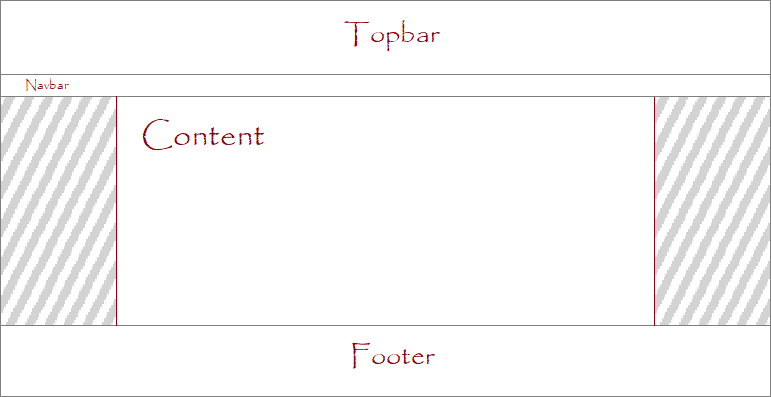
\includegraphics[width=100mm]{images/sketch_1.png}
    \caption{Initial sketch for index.html}
    \end{figure}

    \begin{figure}[H]
    \centering
    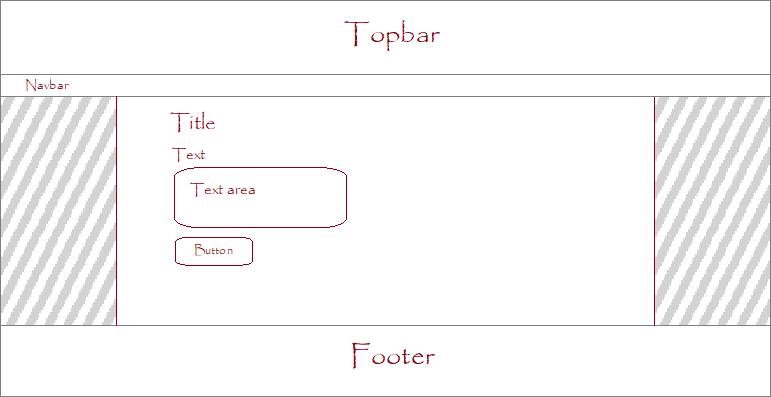
\includegraphics[width=100mm]{images/sketch_2.png}
    \caption{Initial sketch of Cipher Page}
    \end{figure}
    \subsection{The ciphers}
    The ciphers to be implemented:
    \begin{itemize}
    \item Rotate by 13 (ROT13) Encoder.
    \item Base64 Encoder.
    \item Morse Encoder.
    \end{itemize}


    \subsection{The requirements to be fulfilled} 
    \begin{itemize} 
    \item Design will be consistent through all web-pages (for example, same colors or font).
    \item Navigation requirements: 
    \begin{itemize}
    \item A heading on every web-page.
    \item A navigation bar that will allow the user to navigate through the different web-pages. 
    \item A footer on every page. This will include the author name with the due date.
    \end{itemize}
    \item Colors:
    \begin{itemize}
    \item Blue theme. 
    \item Pages shall not have many contrasting colors. 
    \item Text must be clearly visible under \textbf{all} circumstances.
    \end{itemize}
    \item Buttons will change color \textbf{and} change the pointer style when the user hovers over them with their cursor. 
     \end{itemize}

\pagebreak
    \section{Implementation}
    The web-page fulfills the consistency, navigation, color and button requirements. There is a heading on every page, this allows the user to see what page they currently are on. Moreover, there is a footer further fulfilling the requirements stated in     \textbf{Section 2: Software Design}.
    \begin{figure}[H]
    \centering
    
\includegraphics[width=120mm]{images/index.png}
    \caption{Screenshot of the index page}
    \end{figure}
    \textbf{Navigation Bar:} The buttons in the navigation bar change color, as do buttons throughout the web-page. This can also be seen in the design.html web-page. This allows the user to know what button they are about to click, displayed in Figure 4. There is also a \textbf{drop-down menu} within the navigation bar, seen in figure 5. This decision was made because the ciphers belong in one category, and a drop-down allows the ciphers to be in their own section.
    \begin{figure}[H]
    \centering
    
\includegraphics[width=60mm]{images/navbar_hover.png}
    \caption{Navigation Bar Changing Colors}
    \end{figure}

    \begin{figure}[H]
    \centering
    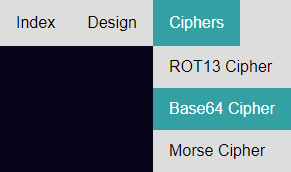
\includegraphics[width=70mm]{images/dropdown_hover.png}
    \caption{Drop-down within navigation bar}
    \end{figure}

    \begin{figure}[H]
    \centering
    
\includegraphics[width=40mm]{images/button_hover.png}
    \caption{Button changing color when hovered}
    \end{figure}


\pagebreak
    \section{Critical Evaluation}
    \subsection{Checklist against plan:} 
        \begin{itemize}   
    \item[\done] Design will be consistent through all web-pages (for example, same colors or font).
    \item Navigation requirements: 
        \begin{todolist}
    \item[\done] A heading on every web-page.
    \item[\done] A navigation bar that will allow the user to navigate the web-page.
    \item[\done] A footer on every page. This will include the author and due date.
        \end{todolist}
 \item Colors:
    \begin{todolist}
    \item[\done] Blue theme. 
    \item[\done] Pages shall not have many contrasting colors. 
    \item[\done] Text must be clearly visible under \textbf{all} circumstances
    \end{todolist}
    \item[\done] Buttons will change color \textbf{and} change the pointer style when the user hovers over them with their cursor. 
        \end{itemize}


    
    \subsection{Possible improvements:}The improvements to be taken into consideration are:
    \begin{itemize}
    \item Add functionality for more ciphers, for example, Vigenere Cipher.
    \item Include images where appropriate. 
    \item Highlight in the navigation bar the current page. This is not so critical because there is already a title in the top bar allowing the user to see the current page.
    \item There is repetitive HTML code, for example, the topbar, navigation bar, footer are all very similar code. The top bar has different text on every page so it's not so critical, also the navbar requires different href links to be placed. However, the footer is the same on every page. Perhaps there is a way to create a footer HTML file which is called upon in the other HTML files, this means that when it is edited once it is edited everywhere. 
    \item Have a tested mobile version of this website.
    \end{itemize} 





    \section{Personal Evaluation} 
    This section will take the opportunity to not only reflect on what I learned but also the challenges I faced, the methods I used to overcome these challenges, and how I feel that I performed.
    \subsection{Lessons Learned} Through the use of HTML, CSS, and Javascript I was able to make an interactive website from scratch. Examples of lessons learned include section off items inside the browser window, allow buttons/cursor to change their appearance when hovered on, create classes in CSS, or use JavaScript to build ciphers.

    \subsection{The Challenges that I Faced}
    Before starting the Web Technologies (SET08101) module at Napier, I had \textbf{no} experience with HTML, CSS, or JavaScript. This posed me with a \textbf{very} steep challenge at the start. Not only because I do not come from a design background, but also my lack of knowledge with the tools put me in a compromising position. I struggled greatly even coming up with a base design and even once I had, the lack of knowledge meant that I was not able to turn my ideas into reality. 
\pagebreak
    \subsection{The Methods that I used to Overcome the Challenges} Initially I made a list of requirements (as seen in \textbf{Section 2.4}). This did not help much as I did not know how to put them into practice. \\\\I often resorted to pages which I liked the design of and analyzed \textbf{why} I liked them. I liked pages that had \textbf{headers and footers}. I liked pages that had \textbf{padding on the right and left side} of the page and that the text did \textbf{not} just span across the screen - this makes a web-page look low effort in my opinion. I liked pages that had \textbf{easy navigation}. To build on this I watched tutorials on how to use CSS to my advantage, and create a website that filled the requirements of my web-page. From this, I sketched out some thoughts (as seen in \textbf{Section 2.2}).
    \subsection{Evaluation of my Performance}  I started with \textbf{zero} knowledge which I did not like, but I wanted to make a difference and I used this opportunity to change that. I feel that I was very focused on the goal from the start. I did not leave this until the last minute. I finished the cipher functionality my project well before the deadline, which allowed me enough time to tweak the website / adjust it to make it how it is now. Personally, I feel like I put a \textbf{lot} of effort into this project and therefore got a lot of experience out of it.



%    \section{Formatting}
%/subsection{Code Listing}
%    You can embed segments of code directly. 
%    \lstinputlisting[caption = Example short python script of code]{./sourceCode/hello.py}
%    \paragraph{Referencing}
%    You should cite References like this: \cite{Keshav}. The references are saved in an external .bib file, and will automatically be added to the bibliography at the end once cited.
    
	
    
%\subsection{PseudoCode}

%\begin{algorithm}[h]
%\For{$i = 0$ \KwTo $100$}{
%print\_number = true\;
%\If{i is divisible by 3}{
% print "Fizz"\;
% print\_number = false\;
%}
%\If{i is divisible by 5}{
% print "Buzz"\;
% print\_number = false\;
%}
%\If{print\_number}{
%    print i\;
%}
%print a newline\;
%}
%\caption{FizzBuzz}
%\end{algorithm}
	
%\section{Conclusion}	
%\bibliographystyle{ieeetr}
%\bibliography{references}
		
\end{document}